\documentclass{article}
\usepackage[utf8]{inputenc} % Permite el uso de caracteres del Español
\usepackage{graphicx}
\usepackage{wrapfig}
\usepackage{subfig}
\usepackage{hyperref}

% set font encoding for PDFLaTeX or XeLaTeX
\usepackage{ifxetex}
\ifxetex
  \usepackage{fontspec}
\else
  \usepackage[T1]{fontenc}
  \usepackage[utf8]{inputenc}
  \usepackage{lmodern}
\fi

% used in maketitle
\title{Reporte Actividad 3: Sondeos meteorológicos de la Atmósfera}
\author{Melissa Matrecitos Avila}
\date{14 de Febrero de 2018}


\begin{document}
\maketitle
\section{Introducción}
En el siguiente trabajo es el reporte de la actividad 3 del curso de Física Computacional, en el cual se analizaron los datos obtenidos de sondeos atmósforicos de la estación de Lindenberg, Alemania. Los datos fueron descargados del sito web de la Universidad de Wyoming, de los cuales se analizaron presión, temperatura, temperatura de rocío, humedad relativa, y  dirección del viento, todos con respecto a la altura del globo meteorológico. Además solo se analizaron los datos correspondientes a los días 22 de Junio de 2017 y 22 de Diciembre de 2017.

La parte fundamental de la práctica es seguir practicando el lenguaje de Python, trabajar con datos en Pandas y crear gráficas de los datos en Matplotlib, todo esto en el entorno de Jupyter Notebook.

A continuación se mostrarán los fundamentos o conceptos básicos del tema, a analizar, también el análisis de los datos que se obtuvieron, los resultados a los que se llegaron y por supuesto la conclusión de la actividad.

\section{Fundamentos}
Cómo se mencioinó en prácticas pasadas, la atmósfera de la Tierra es una capa de gases, conocida comúnmente como aire, que rodea la Tierra y es retenida por la gravedad del planeta. Ésta se puede dividir en cinco capas principales, que son la exosfera, la troposfera, la estratosfera, la mesosfera y la termosfera. Debido a que cada capa tiene distintas características físicas dependientes de la altura, es de gran importancia medir algunas de estas caracteríticas, lo cual se logra por medio de sondeos de globo instrumentados.

Un sondeo atmosférico es una medición de la distribución vertical de las propiedades físicas de la columna atmosférica, como presión, temperatura, velocidad y dirección del viento además de otras propiedades. Tales mediciones se realizan en una variedad de formas que incluyen detección remota y observaciones in situ. Para realizar los sondeos, se utilizan los globos meteorológicos los cuales transportan instrumentos hacía la atmósfera para enviar información sobre las propiedades mencionadas anteriormente.


\section{Análisis de datos}
Antes de realizar las gráficas, fue necesario "limpiar" los datos, es decir, darles formato, ya que el que tenían no era el adecuado para trabajar con ellos. 
A continuación se muestran los pasos que se siguieron para dar formato a los datos. Solo se muestra lo correspondiente a una fecha, ya que se les hizo lo mismo a ambas fechas.
Lo primero que se hizo (además de exportar las bibliotecas), fue leer los datos, saltandose las dos primeras lineas, para después no leer de los renglones 0 y 1, como se muestra en la imagen de abajo:

\begin{center}
    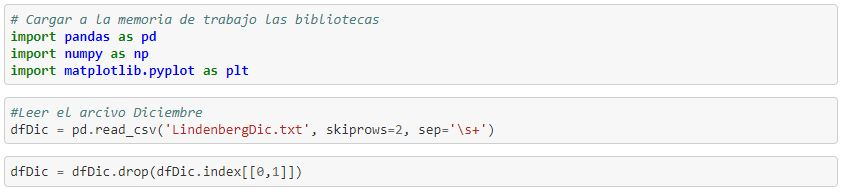
\includegraphics[width=0.85\textwidth]{LeerDatos.JPG}
\end{center}

Posteriormente se evitaron leer los últimos 30 datos, ya que cotenían las referencias de la estación y no del sondeo.
\begin{center}
  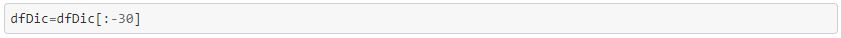
\includegraphics[width=0.85\textwidth]{BorrarDatos.JPG}
\end{center}
Después de tener los datos con el formato deseado, se le cambo su tipo a para poder graficarlos, esto se logro, definiendo un conjunto con los nombres de las columnas y cambiar el tipo del conjunto:
\begin{center}
  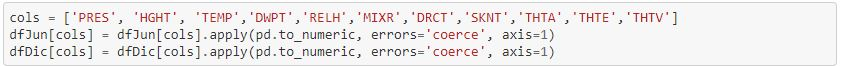
\includegraphics[width=0.85\textwidth]{Objeto.JPG}
\end{center}

Para finalizar se realizaron las gráficas de los datos, a continuación se muestra un ejemplo de cómo se hizo:
\begin{center}
  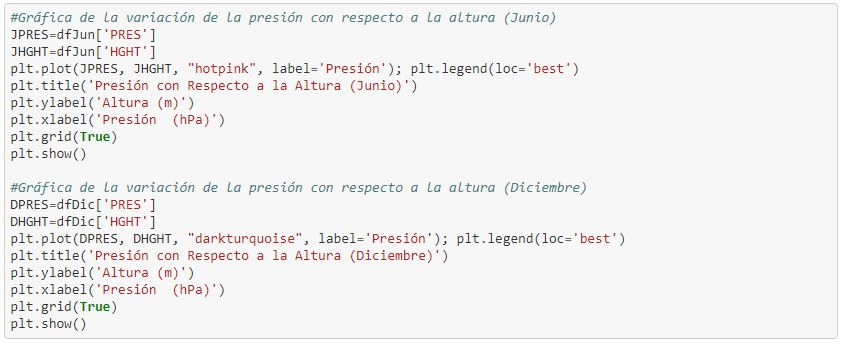
\includegraphics[width=0.85\textwidth]{Grafica.JPG}
\end{center}

\section{Resultados}
En esta sección se muestrán las gráficas resultantes al comparara algunas propiedades físicas con la altura.

\textbf{Gráfica de la variación de la presión con respecto a la altura}
\begin{center}
    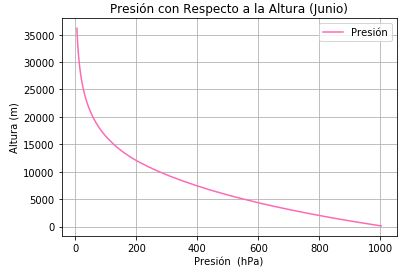
\includegraphics[width=0.4\textwidth]{PresionJ.JPG}
    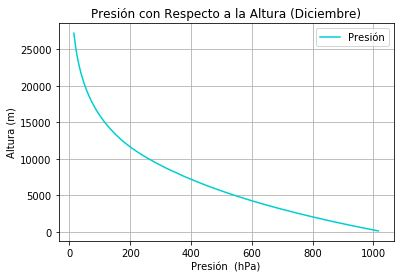
\includegraphics[width=0.4\textwidth]{PresionD.JPG}
\end{center}
Se observa como las gráficas son muy parecidas, independientemente de la fecha en la que se realizó el sondeo, además de que cumplen con lo visto en el curso de Fluidos y Fenómenos Térmicos: conforme la altura aumenta, la presión atmósferica disminuye.

\textbf{Gráfica de temperatura como función de la altura}
\begin{center}
    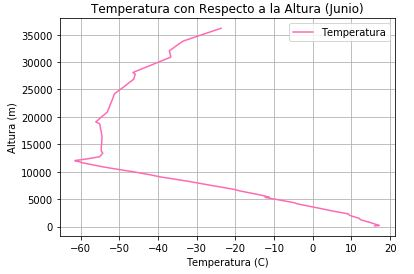
\includegraphics[width=0.4\textwidth]{TempJ.JPG}
    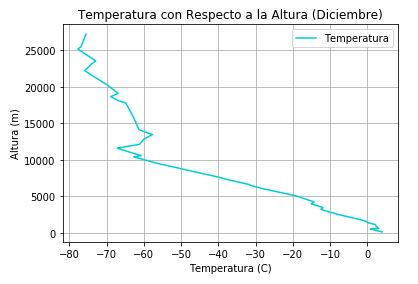
\includegraphics[width=0.4\textwidth]{TempD.JPG}
\end{center}
En la gráfica se ve como la temperatura es más baja conforme la altura aumenta, hasta una altura de aproximadamente de 12 km, donde se nota un cambio brusco en esta. A esa altura se encuentra la tropopausa, la cual es la zona de transición entre la troposfera y la estratosfera.

\textbf{Gráfica de la temperatura y temperatura de rocío, como función de la altura}
\begin{center}
    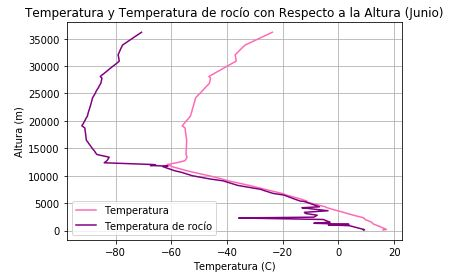
\includegraphics[width=0.4\textwidth]{RocioJ.JPG}
    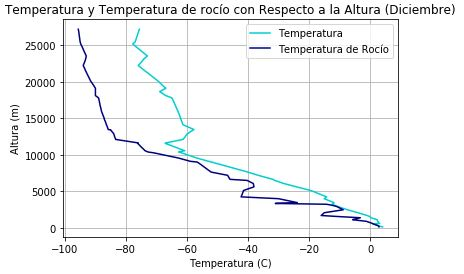
\includegraphics[width=0.4\textwidth]{RocioD.JPG}
\end{center}
El punto de rocío o temperatura de rocío es el valor al que debe descender la temperatura del aire para que el vapor de agua existente comience a condensarse. Por lo tanto ésta es menor a la temperatura del ambiente.
Cómo se muestra en las gráficas, la temperatura del ambiente es mayor que la temperatura de rocío y la diferencia de éstas es más notable en el mes de Junio. Además estas siguen disminuyendo conforme la antura aumenta.

\textbf{Gráfica de la rapidez de los vientos en nudos}
\begin{center}
    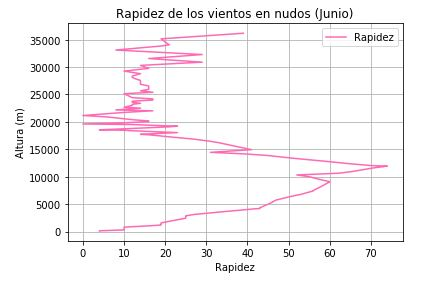
\includegraphics[width=0.4\textwidth]{RapidezJ.JPG}
    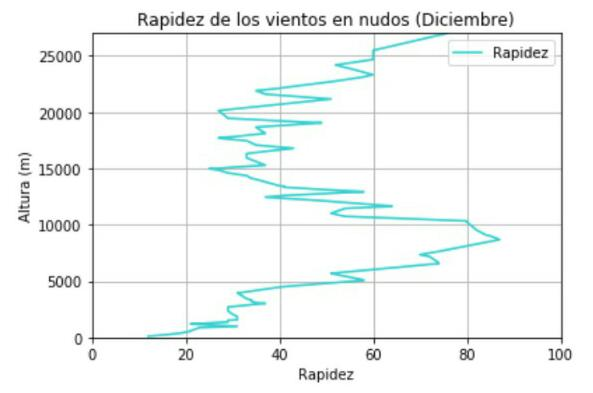
\includegraphics[width=0.4\textwidth]{RapidezD.JPG}
\end{center}
La gráfica muestra como el viento varía más entre más alto se encuentre, lo cual se puede originar debido, a la diferencia de temperaturas que hay en lo alto de la atmósfera.

\textbf{Gráfica de la humedad relativa como función de la altura}
\begin{center}
    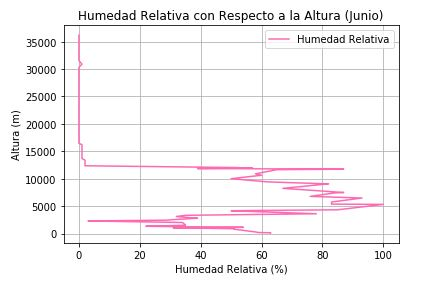
\includegraphics[width=0.4\textwidth]{HumedadJ.JPG}
    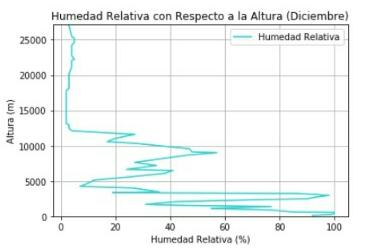
\includegraphics[width=0.4\textwidth]{HumedadD.JPG}
\end{center}
Al igual que en las gráficas de temperatura, se nota un cambio drástico a la altura de la tropopausa, por debajo de esta se ven muchos cambios en la humedad, pero después se mantiene prácticamente constante y muy pequeña. Ademas esto pasa independientemente de la fecha.

\section{Conclusión}
Me gustó mucha la actividad por que nunca me había enfrentado a una situación de este tipo, donde fuera más laborioso ajustar la lectura de datos que hacer las gráficas, ya que las gráficas se hacían todas casi de la misma manera, solo cambiaban las variables con las que se iba a trabajar, mientras que los datos había que revisar cuales erán datos del sondeo, cuales de la estación y sobre todo el encabezado, ya que éste provocaba que los datos fueran de tipo object, del cual no se pueden hacer graficas.

Considero que también influyó el hecho de que en la práctica pasada ya se habían trabajado con gráficas, mientras que no habíamos visto nada del ajuste de datos, por lo que se tuvo que hacer una búsqueda para encontrar los comandos necesarios.

\section{Bibliografía}
\begin{itemize}
\item Columns, p. (2018). pandas: to numeric for multiple columns. Stackoverflow.com. Recuperado el 7 Febrero 2018, de \url{https://stackoverflow.com/questions/36814100/pandas-to-numeric-for-multiple-columns}

\item color example code: named colors.py — Matplotlib 2.0.2 documentation. (2018). Matplotlib.org. Recuperado el 12 Febrero 2018, de \url{https://matplotlib.org/examples/color/named_colors.html}

\item Atmospheric sounding. (2018). En.wikipedia.org. Recuperado el 13 Febrero 2018, de \url{https://en.wikipedia.org/wiki/Atmospheric_sounding}

\item Weather balloon. (2018). En.wikipedia.org. Recuperado el 13 Febrero 2018, de \url{https://en.wikipedia.org/wiki/Weather_balloon}

\item Atmosphere of Earth. (2018). En.wikipedia.org. Recuperado el 13 Febrero 2018, de \url{https://en.wikipedia.org/wiki/Atmosphere_of_Earth}

\end{itemize}

\section{Apéndice}
\begin{enumerate}
\item¿Cuál es tu opinión general de esta actividad?

Me gustó por que nunca me había enfrentado a situaciones de este tipo.

\item¿Qué fue lo que más te agradó? ¿Lo que menos te agradó?

Me gustó lo fácil que es hacer las gráficas y por supuesto el darles formato. Lo que no me gustó fue que aún no me puedo acostumbrar a hacer el reporte en Latex.

\item¿Que consideras que aprendiste en esta actividad?

Aprendpí la importancia de revisar los datos y como editar la lectura de una manera más sencilla.

\item¿Qué le faltó? ¿O le sobró?

Me pareció una actividad muy completa, no considero que le haga falta o sobre algo.

\item¿Que mejoras sugieres a la actividad?

Me parece bien así como esta.
\end{enumerate}

\end{document}
